% This file was converted to LaTeX by Writer2LaTeX ver. 1.6.1
% see http://writer2latex.sourceforge.net for more info
\documentclass[11pt]{article}
\usepackage{amsmath,amssymb,amsfonts}

%\usepackage[a4paper, total={17cm, 26cm}]{geometry}
\usepackage[a4paper,margin=1.5cm]{geometry}
\usepackage{color}
\usepackage{hyperref} % Pour liens internets cliquables
\hypersetup{
    colorlinks=true,
    linkcolor=blue,
    filecolor=magenta,      
    urlcolor=blue, %cyan
    pdftitle={Cours de physique - DLPP - 2022},
    pdfpagemode=FullScreen,
    }

\usepackage{hyperref}
\usepackage[
    type={CC},
    modifier={by-nc-sa},
    version={3.0},
]{doclicense}

\usepackage{multicol}
\setlength{\columnsep}{0.5cm}
\def\columnseprulecolor{\color{black}}

% pour les pieds de page et entêtes
\usepackage{fancyhdr}

\pagestyle{fancy}
\fancyhf{}
\lhead{Cours de physique}
\rhead{Oscillateur harmonique}
\lfoot{En cours de rédaction et correction - ne pas distribuer - \ccbyncsa}
\rfoot{Page \thepage}

\usepackage{fontspec}
\usepackage{xunicode}
\usepackage{xltxtra}
\usepackage{array}
\usepackage{hhline}
\usepackage{graphicx}
\usepackage{polyglossia}
\setdefaultlanguage{french}

\newcounter{Text}
\renewcommand\theText{\arabic{Text}}
\title{Cours de physique de $6^e$ secondaire - 2021-2022 \\
En cours de rédaction et correction - ne pas distribuer \\
tout commentaire bienvenu par email à \\
 manueldephysique@educode.be}
\author{Alexandra David - Corinne Leyssen - Nicolas Pettiaux - Matteo Poncé}

\begin{document}
\maketitle
\doclicenseThis

\setcounter{tocdepth}{10}
\renewcommand\contentsname{Table des matières}
\tableofcontents

\hrulefill

\begin{multicols}{2}

\section{Énergie de l’oscillateur harmonique}

\subsection{Vidéos à regarder}
\begin{enumerate}
\item \href{https://videos.domainepublic.net/w/k4SYtXTppaRqy5fQQV3foV}{Bilan énergétique de l'oscillateur horizontal}
\item \href{https://videos.domainepublic.net/w/k19sGJLazDaDXk2Xvz2HpX}{Énergie d'un oscillateur masse-ressort horizontal}
\end{enumerate}

\subsection{Différentes formes d’énergie d’un oscillateur harmonique}
\begin{enumerate}
\item Energie cinétique~(due à la vitesse) :  $E= \frac{1}{2} mv^2$
\item Energie potentielle gravifique~(due à la hauteur) :  $E=mgh$
\item Energie potentielle élastique~(due à la compression ou dilatation d’un ressort) $E=\frac{1}{2} ky^2$ 
\end{enumerate}

\subsection{Energie totale d’un oscillateur harmonique}
L’énergie totale mécanique d’un oscillateur harmonique est la somme des énergies cinétique et potentielle (gravifique
pour un pendule simple et élastique pour un ressort horizontal).

Dans le cas où les frottements sont négligés, l’énergie totale reste constante (principe de conservation d’énergie). 

Exprimons mathématiquement ce principe en répondant à la question : 

En toute généralité, quelle est l’énergie totale d’un oscillateur harmonique~ (que ce soit un pendule simple ou un
pendule élastique) ? 

Lorsqu’un oscillateur harmonique est à une position extrême (+A ou  -A), l’énergie cinétique est nulle et l’énergie
potentielle maximale (énergie potentielle gravifique pour un pendule simple et énergie potentielle élastique pour un
ressort horizontal).

De même, pour un oscillateur harmonique (quel qu’il soit), lorsque la vitesse est maximale, l’énergie potentielle est
nulle (énergie potentielle gravifique pour un pendule simple et énergie potentielle élastique pour un ressort
horizontal). L’énergie totale de l’OH ($E_T$) est donc égale à $E=\frac{1}{2}mv_{\text{max}}^2$   

Or nous savons que  :  $E_{\text{T}}=\frac{1}{2}m v_{\text{max}}^2$  avec   $v_{\text{max}}=A\omega $. Donc 
$E_{\text{T}}=\frac{1}{2}mv_{\text{max}}^2=\frac{1}{2}mA^2\omega ^2$

Or  $T$  et  $\omega $  ne varient pas au cours de l’oscillation, elles sont constantes.

Notons $k=m\omega ^2$ où k est une constante. On trouve $E_{\text{totale}}=\frac{1}{2}kA^2$ 
qui est donc l’énergie totale d’un oscillateur harmonique. 


\subsection{Que représente k ? }
L’énergie totale d’un oscillateur harmonique est~ $E_{\text{T}}=\frac 1 2kA^2$ : 

Que représente physiquement cette constante  $k=m\omega ^2$?

Pour un pendule élastique (un ressort)

k est la constante de raideur du ressort  $F=kx$(loi de Hooke) où  $x$~étant l’allongement du ressort à l’équilibre
lorsque ce dernier est soumis à une force de traction (ou de compression) F.

Pour un pendule simple $k=m\omega ^2$  $\omega =2\frac{\pi } T$ et  $T=2\pi \sqrt{\frac L g}$. Don $\omega
^2=\frac{4\pi ^2}{T^2}=4\pi ^2\frac 1{4\pi ^2}\frac g L=\frac g L$
et  $\omega=\sqrt{\frac{g}{L}}$  où  $L$ est longueur du pendule et  $m$, sa masse.

\subsection[Évolution au cours du temps des énergies cinétique, potentielle et totale. ]{Évolution au cours du temps des
énergies cinétique, potentielle et totale. }
\begin{center}
\begin{minipage}{8.89cm}


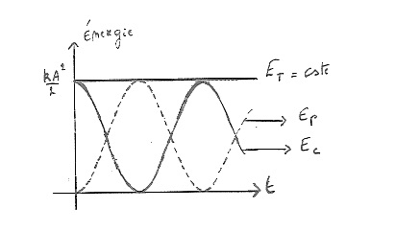
\includegraphics[width=8cm]{COURS2EnergieOHEXERCRESOL-img/COURS2EnergieOHEXERCRESOL-img001.png}
On remarque que lorsque l’énergie cinétique est maximale alors l’énergie potentielle
est nulle et vice versa. Il y a constamment conversion de l’énergie cinétique en potentielle et vice versa, de telle
sorte que l’énergie totale reste constante. 
\end{minipage}
\end{center}

Variation de l’énergie cinétique   $E_c(t)=\frac{1}{2}mv(t)=\frac{1}{2}m\omega ^2A^2\text{cos}^2(\omega t+\phi )$

Variation de l’énergie potentielle  $E_p(t)=\frac{1}{2}\mathit{ky}^2=\frac{1}{2}kA^2\text{sin}^2(\omega t+\phi )$

L’énergie totale reste constante. Elle est égale à la somme des énergies cinétique et potentielle. 

\begin{equation*}
E_c(t)+E_p(t)=E_t=\text{constante}
\end{equation*}


\subsection{Énergie d’un oscillateur harmonique - exercices}

\begin{center}
\begin{minipage}{5.992cm}
 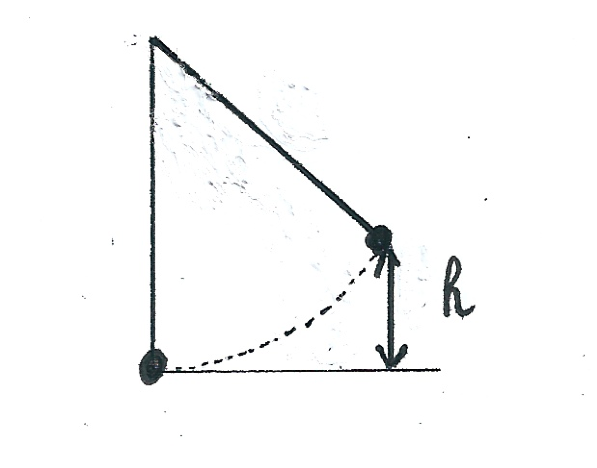
\includegraphics[width=5.457cm,height=4.239cm]{COURS2EnergieOHEXERCRESOL-img/COURS2EnergieOHEXERCRESOL-img002.png} 
\end{minipage}
\end{center}
\subsubsection{Exercice 1}
Un pendule simple de longueur égale à 40 cm et d’une masse de 50 g est lâché lorsqu’il fait un angle de 10° avec la
verticale. 

\begin{enumerate}
\item Calculez son énergie potentielle maximale.
\item Calculez sa vitesse maximale.
\item Calculez sa vitesse à mi-hauteur. 
\item Quelle est son énergie totale ? 
\end{enumerate}
\subsubsection[Exercice 2]{Exercice 2}
\begin{center}
\begin{minipage}{3.81cm}
 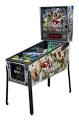
\includegraphics[width=3cm]{COURS2EnergieOHEXERCRESOL-img/COURS2EnergieOHEXERCRESOL-img003.png} 
\end{minipage}
\end{center}
Pour lancer une boule (masse 50 g) de « flipper », on comprime de 10 cm un ressort d’une constante de  raideur égale à
200 N/m. Quelle sera la vitesse de la boule lorsqu’elle aborde le virage au bout d’une course rectiligne de 1,5 m après
qu’elle ait quitté le ressort. Négligez tout frottement !

\begin{enumerate}
\item si le flipper est horizontal ? 
\item s’il fait un angle de 5° avec l’horizontale ?
\end{enumerate}
\subsubsection[Exercice 3]{Exercice 3}
\begin{center}
\begin{minipage}{6.276cm}
 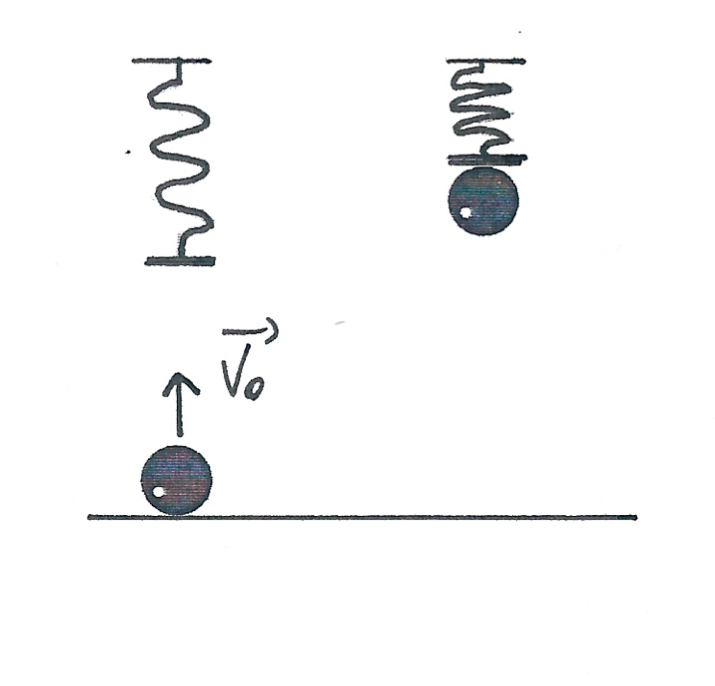
\includegraphics[width=5.75cm,height=5.539cm]{COURS2EnergieOHEXERCRESOL-img/COURS2EnergieOHEXERCRESOL-img004.png} 
\end{minipage}
\end{center}
Une balle de 500g est lancée verticalement vers le haut sur un ressort de constante de raideur égale à 32 N/m et de
masse négligeable. La vitesse de lancer de 2 m/s.

Le ressort se comprime de 12 cm lorsque la bille atteint sa hauteur maximale.

Quelle est la hauteur atteinte par la bille ? 

\subsubsection{Exercice 4}
Un fusil de fléchettes comprend un ressort de raideur k = 250 N/m, de longueur à vide l0 = 12 cm et qui, comprimé par la
fléchette de masse 25 g, ne mesure plus que l = 4,0 cm.

\begin{enumerate}
\item Avec quelle vitesse la fléchette sort-elle du fusil dans le cas d’un tir horizontal. Faire le calcul sans tenir
compte du frottement entre fléchette et fusil.
\item Quelle altitude maximale peut-elle atteindre dans le cas d’un tir vertical ? Faire le calcul sans tenir compte du
frottement entre fléchette et fusil ni de la résistance de l’air.

\end{enumerate}
\subsubsection[Exercice 5]{Exercice 5}
\begin{center}
\begin{minipage}{8.876cm}
 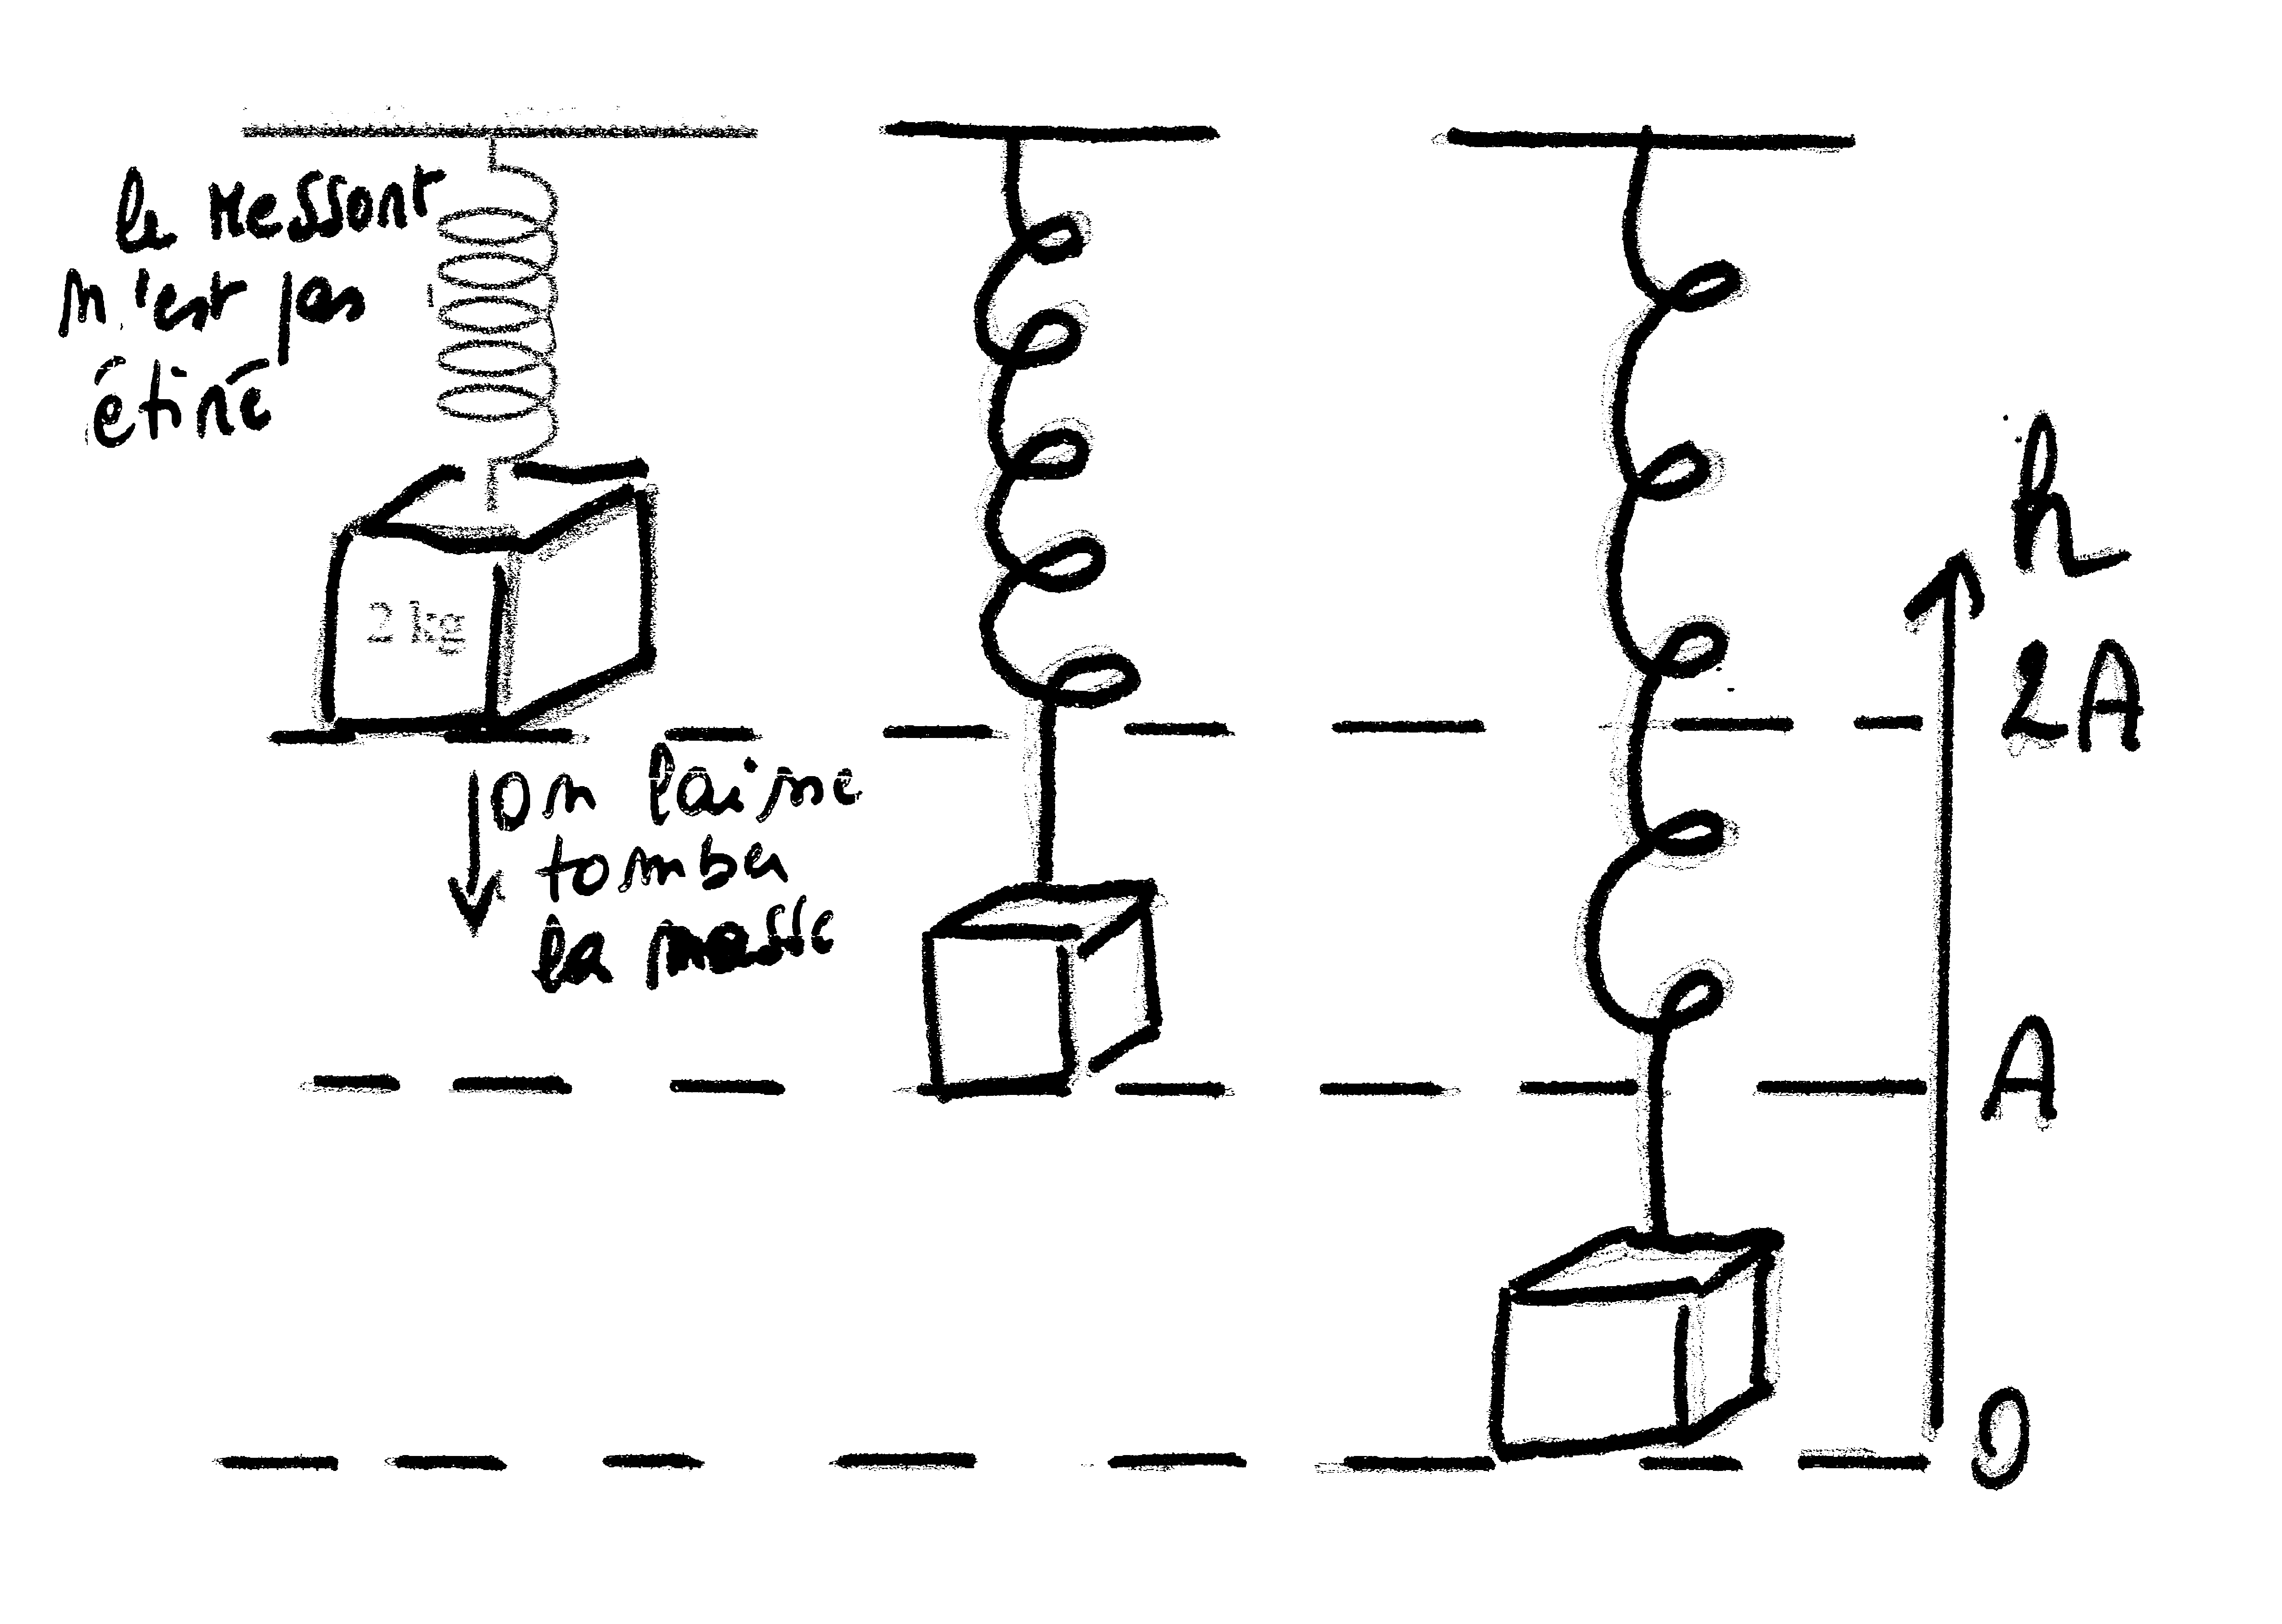
\includegraphics[width=8cm]{COURS2EnergieOHEXERCRESOL-img/COURS2EnergieOHEXERCRESOL-img005.png} 
\end{minipage}
\end{center}
La masse de 2 kg de la figure ci-contre est  suspendue au plafond avec un ressort de masse négligeable et dont la
constante de raideur vaut 200 N/m. Au départ, le ressort n’est pas étiré ni comprimé. On laisse alors tomber la masse
sans la pousser. On aura alors un mouvement d’oscillation de la masse. 

\begin{enumerate}
\item Quelle sera la distance parcourue par le ressort avant qu’il n’entame sa remontée verticale ? 
\item Quelle sera la vitesse maximale du ressort ?  
\end{enumerate}


\begin{center}
\begin{minipage}{3.817cm}
 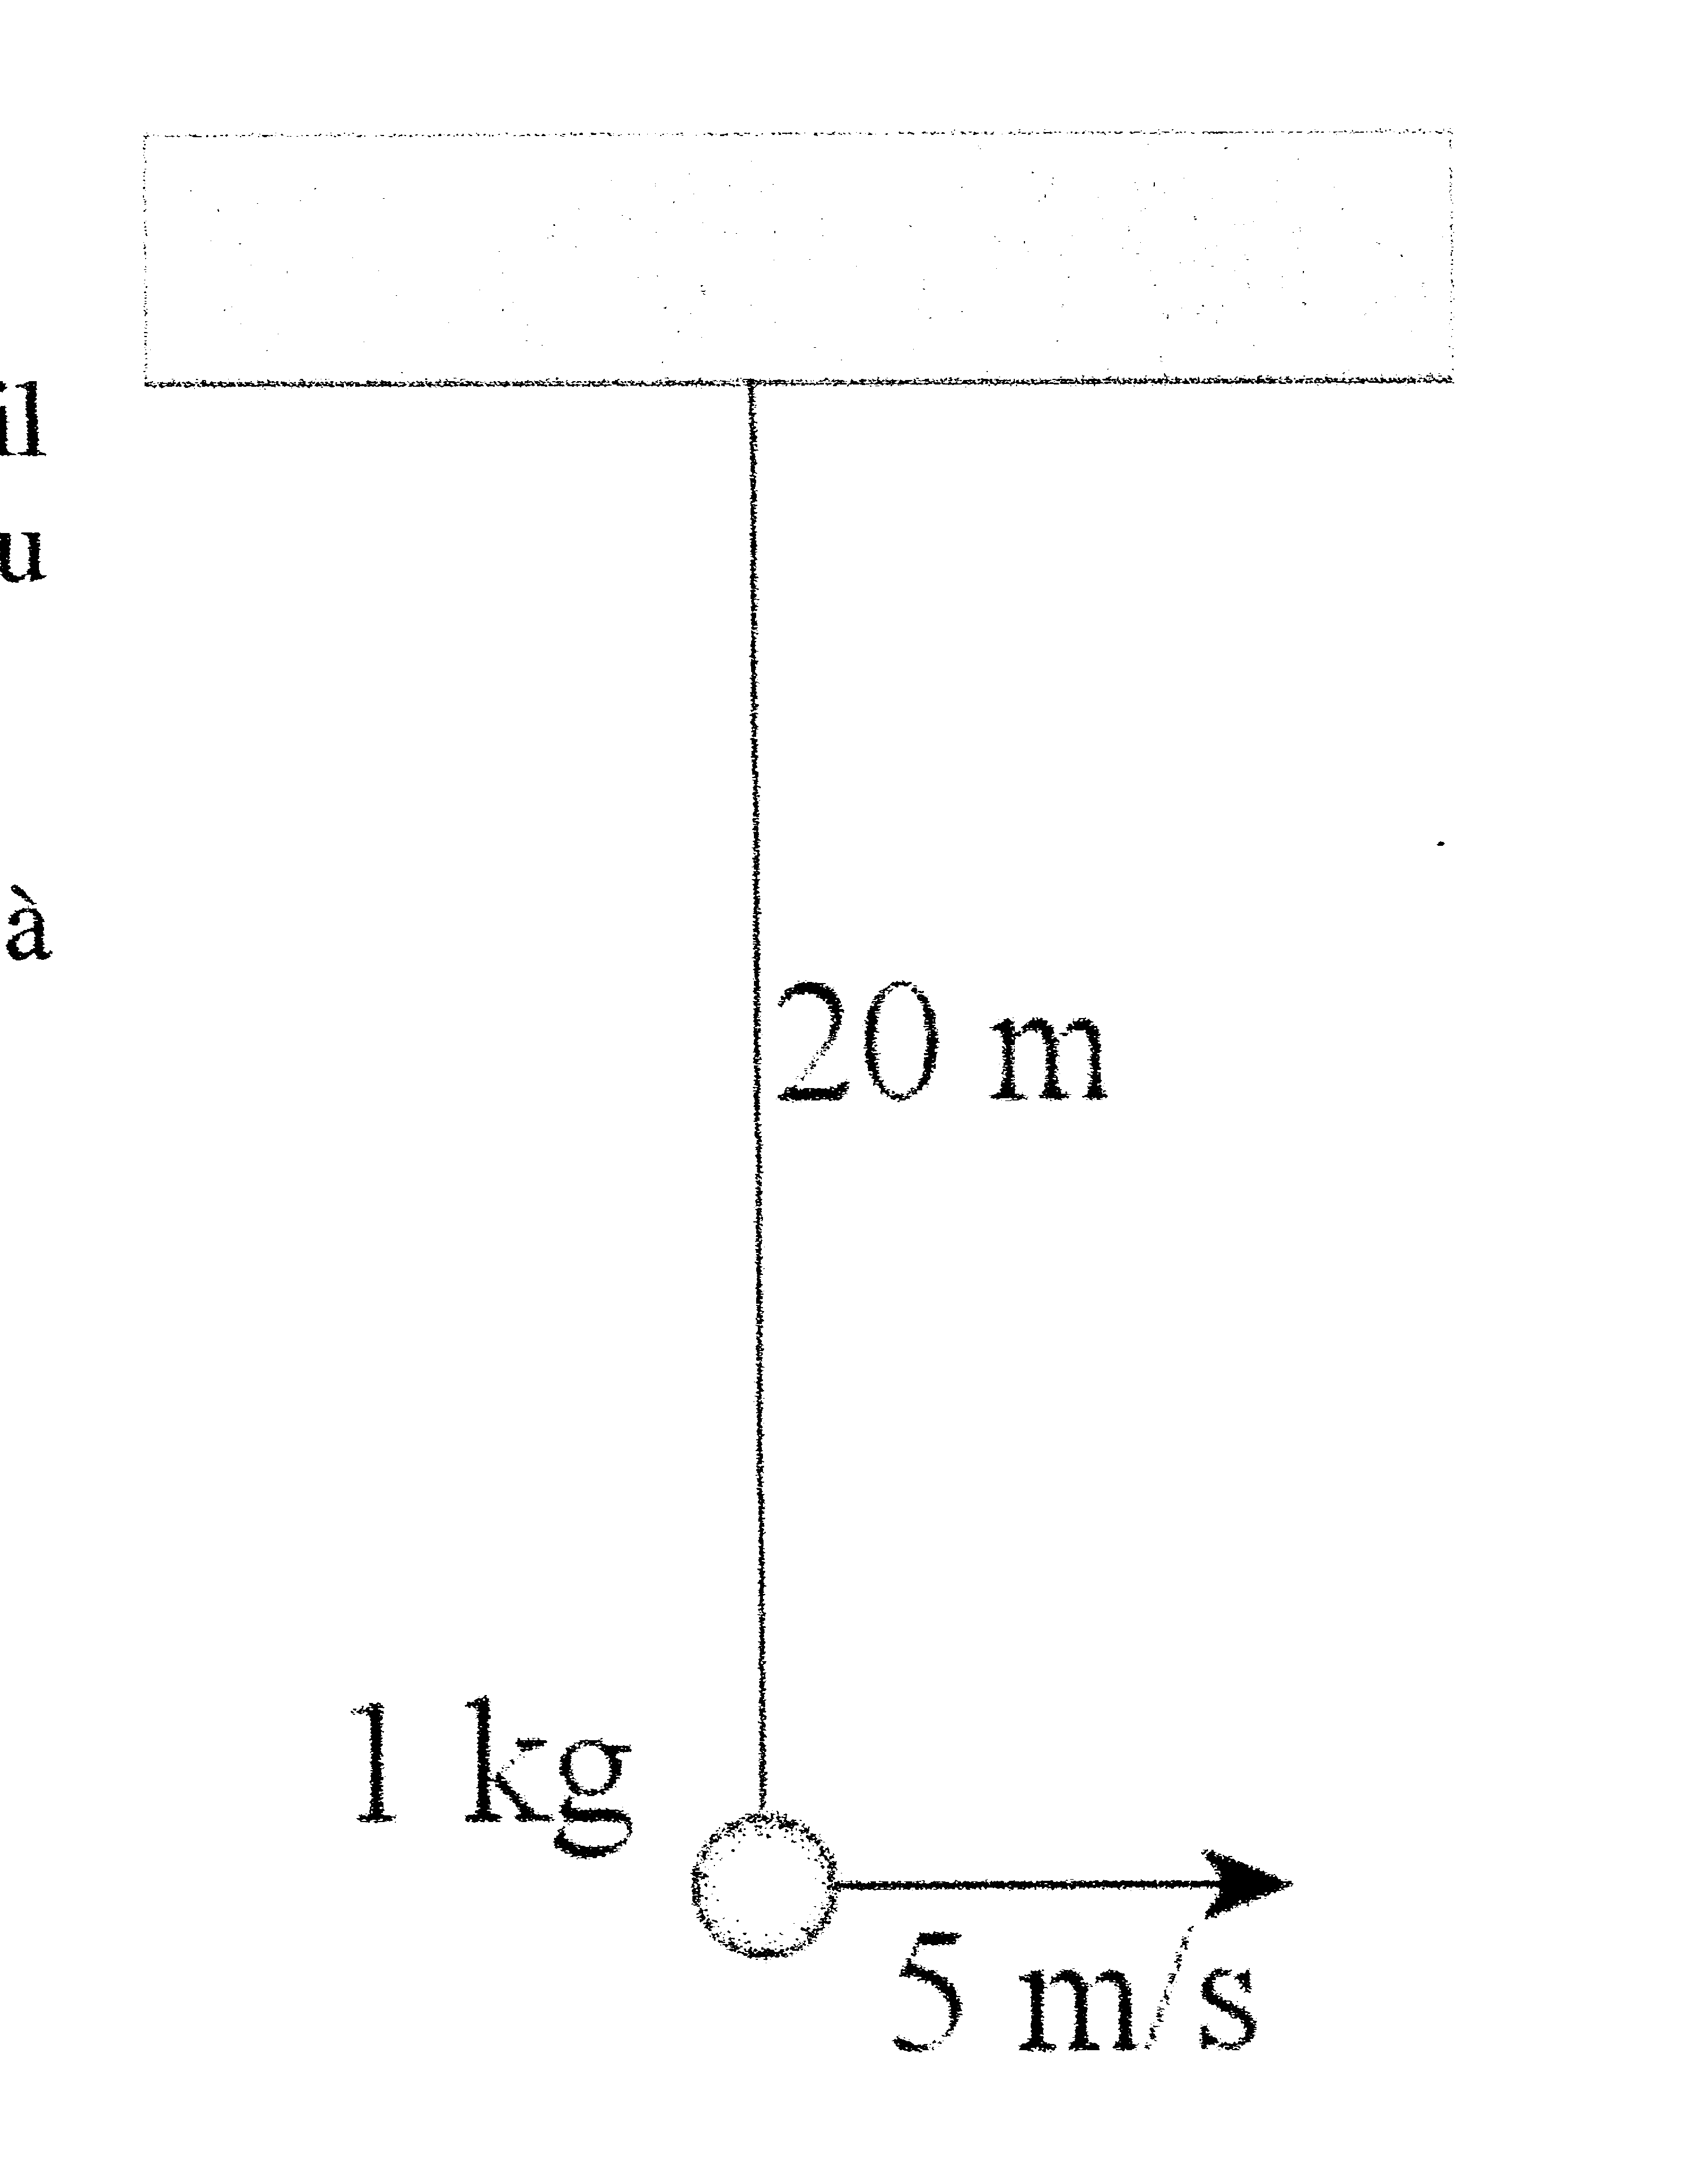
\includegraphics[width=3cm]{COURS2EnergieOHEXERCRESOL-img/COURS2EnergieOHEXERCRESOL-img006.png} 
\end{minipage}
\end{center}
\subsubsection{Exercice 6}
Le pendule de la figure ci-contre est en mouvement harmonique et a une vitesse de 5 m/s quand il passe par sa position
d’équilibre. Quelle est la vitesse du pendule lorsqu’il fait un angle de 10° par rapport à la verticale ? 

\end{multicols}


\section{Résolutions }

 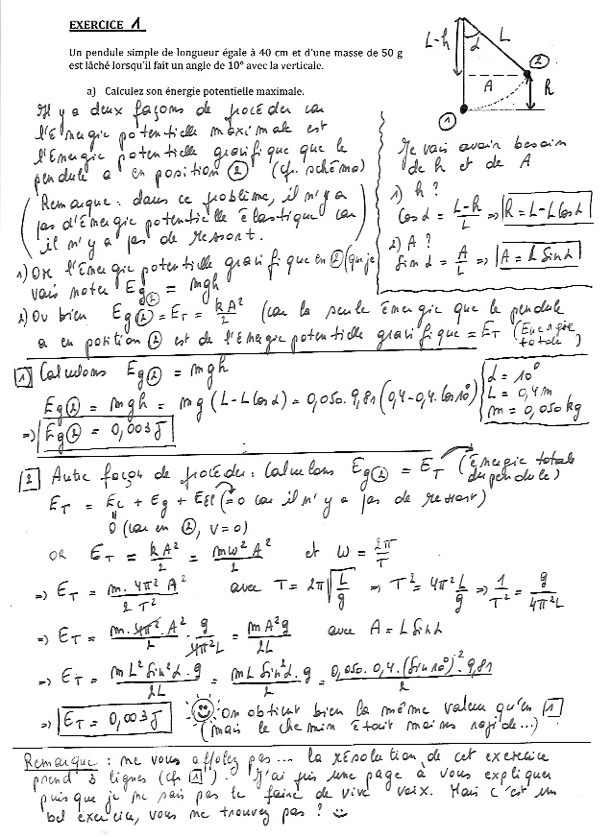
\includegraphics[width=15cm]{COURS2EnergieOHEXERCRESOL-img/COURS2EnergieOHEXERCRESOL-img007.png} 

 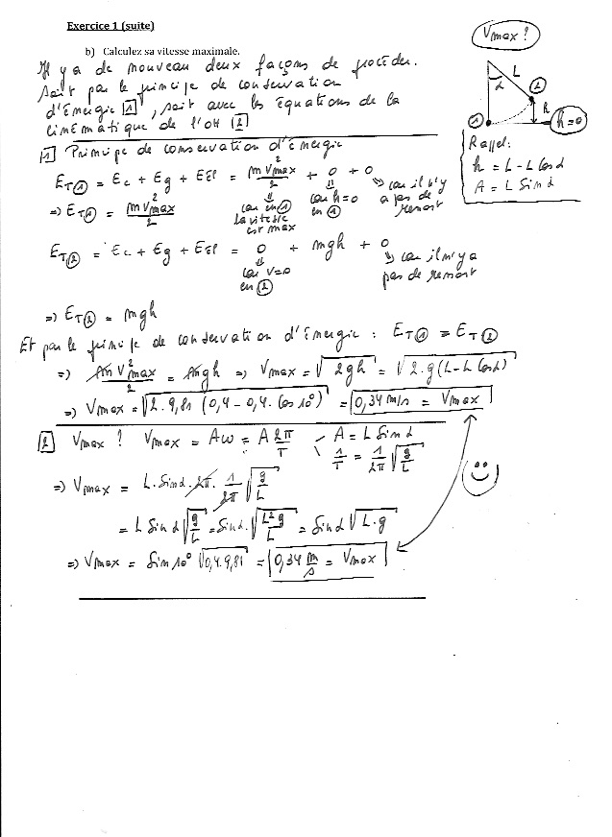
\includegraphics[width=15cm]{COURS2EnergieOHEXERCRESOL-img/COURS2EnergieOHEXERCRESOL-img008.png} 

 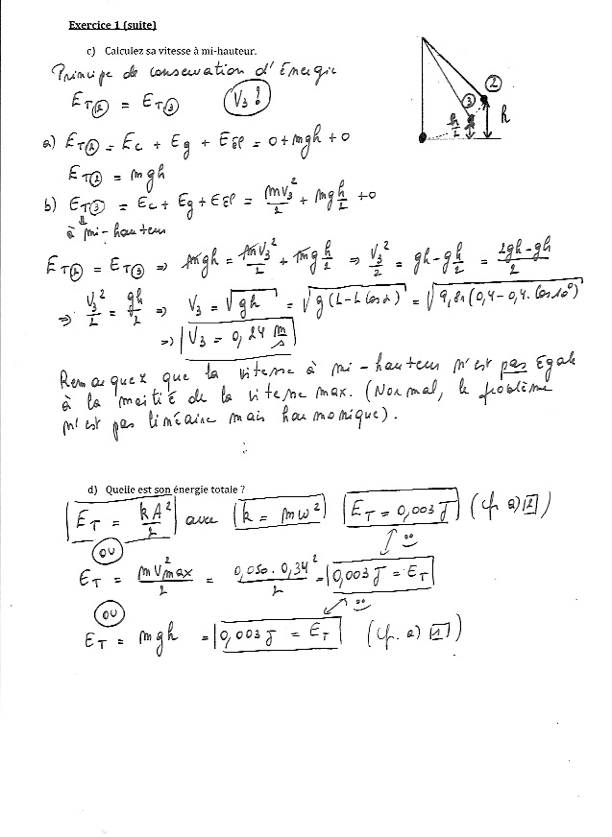
\includegraphics[width=15cm]{COURS2EnergieOHEXERCRESOL-img/COURS2EnergieOHEXERCRESOL-img009.png} 

 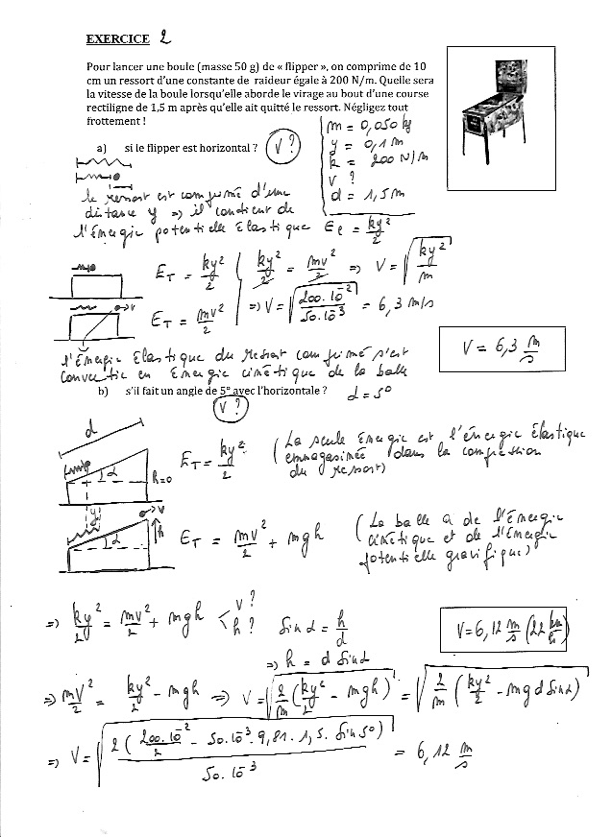
\includegraphics[width=15cm]{COURS2EnergieOHEXERCRESOL-img/COURS2EnergieOHEXERCRESOL-img010.png} 

 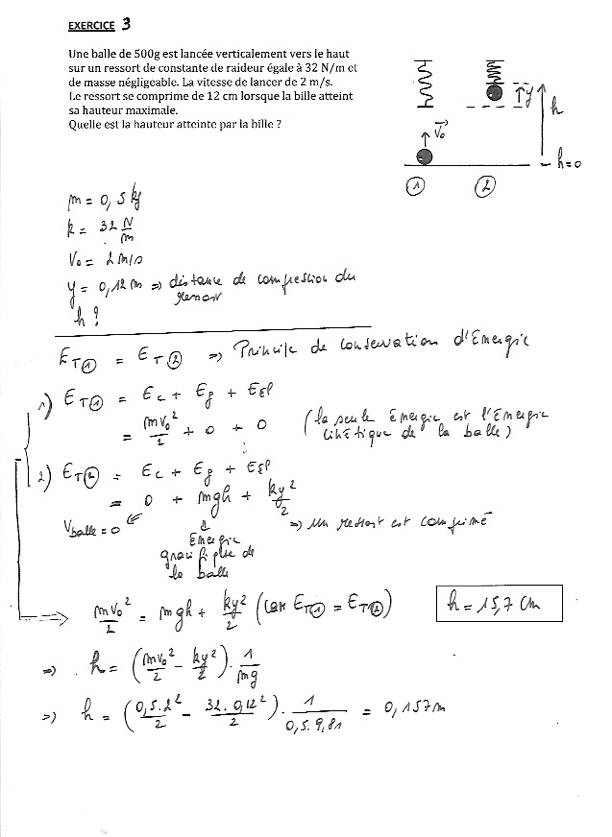
\includegraphics[width=15cm]{COURS2EnergieOHEXERCRESOL-img/COURS2EnergieOHEXERCRESOL-img011.png} 

 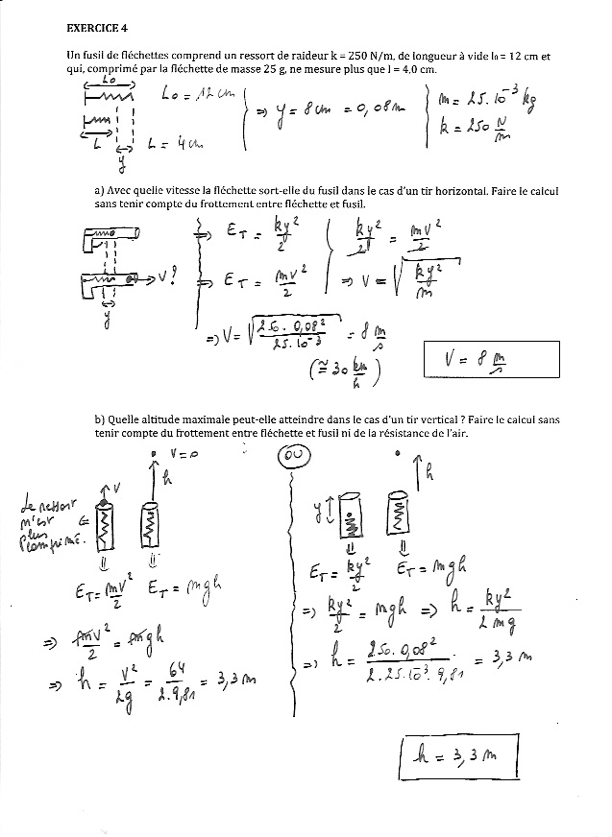
\includegraphics[width=15cm]{COURS2EnergieOHEXERCRESOL-img/COURS2EnergieOHEXERCRESOL-img012.png} 

 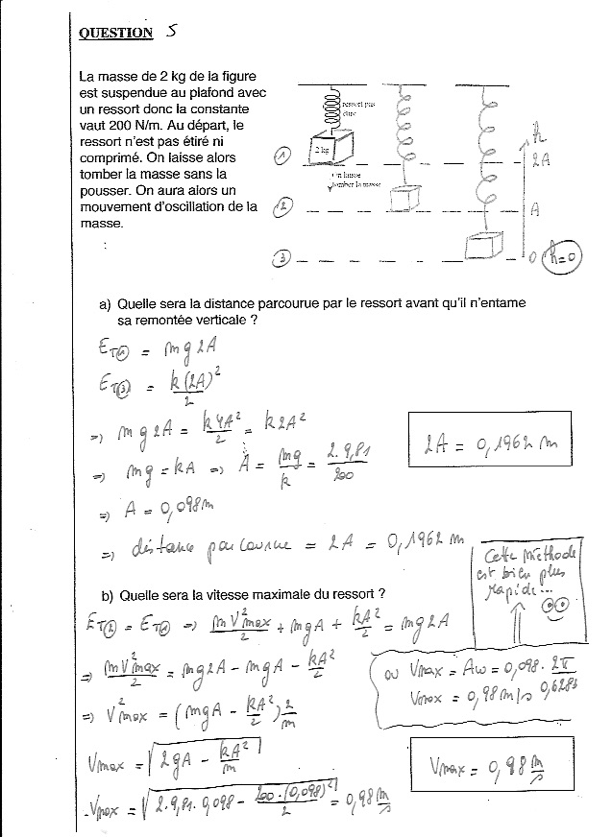
\includegraphics[width=15cm]{COURS2EnergieOHEXERCRESOL-img/COURS2EnergieOHEXERCRESOL-img013.png} 

 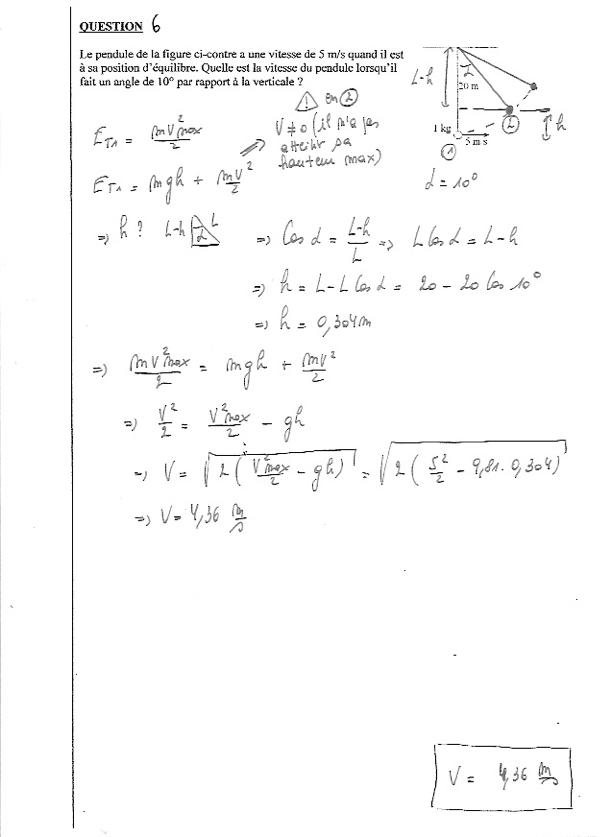
\includegraphics[width=15cm]{COURS2EnergieOHEXERCRESOL-img/COURS2EnergieOHEXERCRESOL-img014.png} 
\end{document}
